\documentclass[a4paper,10pt]{report}
\usepackage[utf8]{inputenc}
\usepackage[english,czech]{babel}
\usepackage{makeidx}
\usepackage{url}
\usepackage{tikz}
\usepackage{float}
\usepackage{pdfpages}
\usepackage{amsfonts}
\usepackage{mdwlist}
\usepackage{xcolor}
\usepackage{listings}
\usepackage[utf8]{inputenc}
\usepackage[T1]{fontenc}
\usepackage{listingsutf8}
\usepackage{cite}
\usepackage{mdframed}
\usepackage{float}

\begin{document}
\title{Úloha ZBS: zobecněná bisekční šířka}
\author{Pavel Verner \\ Martin Beránek}
\maketitle

\tableofcontents
\listoffigures
\listoftables
\newpage

\section{Definici problému}

\subsection{Vstupní data}

\begin{description}
	\item[a] -- přirozené číslo,
	\item[n] -- přirozené číslo představující počet uzlů grafu G, $5 \leq n$,
	\item[m] -- přirozené číslo představující počet hran grafu G, $n \leq m$,
	\item[k] -- přirozené číslo řádu jednotek představující průměrný stupeň uzlu grafu G, $3 \leq k \leq n$,
	\item[$G(V,E)$] -- jednoduchý souvislý neorientovaný neohodnocený graf o n uzlech a m hranách.
\end{description}

\subsection{Úkol}

Naleznout rozdělení množiny n uzlů grafu G do dvou disjunktních podmnožin X a Y tak, že podmnožina X obsahuje a uzlů, podmnožina Y obsahuje $n-a$ uzlů $a$ počet všech hran $\{u,v\}$ takových, že u je z X a v je z Y, je minimální.

\subsection{Výstup algoritmu}

Výpis disjuktních množin uzlů X a Y a počet hran tyto množiny spojující.

\subsection{Popis vstupu}

Algoritmus dostává na vstup matici přechodů s číslem $a$. Matice je generována z aplikace \texttt{generator}, ta vytvoří matici na základě zadané elikosti a stupně grafu. Následně je na výsledek uplatněna aplikace \texttt{souvislost}, ta má za cíl z nesouvislého grafu vygenerovat souvislý graf.

\section{Generování stavového prostoru}

Pro vytvoření množin podgrafu je použita rekurzivní funkce, která vkládá stavy do zásobníku. Při generování prochází strom možných vrcholů spadajících do podgrafu X. Při vytvoření podmnožiny velikosti \texttt{a} vloží množinu na zásobník. Příklad pro $n=5$ a $a=4$ je na obrázku \ref{fig:com}.

\begin{figure}[H]
  \centering
    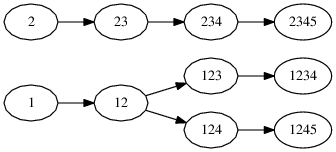
\includegraphics[width=0.5\textwidth]{a45.png}
  \caption{Příklad vytvoření podmnožiny velikosti 4 z grafu s počtem vrcholů 5}
  \label{fig:com}
\end{figure}


Z obrázku jasně vyplývá, že počet podmnožin se bude rovnat při $n$ a $a$ přesně ${n\choose a}$.

Funkce, která kombinace vytváří, prochází postupně celý strom, provede přesně následující počet kroků:

\hspace{1cm}

$\Theta(n) = \sum^{n-a+1}_{i=0}\sum^{i}_{j=0} (a-1) + (2a-n)\cdot j$

\hspace{1cm}

tedy

\hspace{1cm}

$O(n) \simeq n^2$

\hspace{1cm}

\section{Popis sekvenčního algoritmu a jeho implementace}

Sekvenční algoritmus je typu \texttt{BB-DFS} (Branch-and-bound Depth-first search). Při hledání stavového prostoru hledáme nejmenší cenu řešení. Není možné žádné stavy vynechat. Počáteční cena je nastavena na nekonečno (přesněji \texttt{UINT\_MAX}).

Implementace je popsána v následujícím pseudokódu:

\begin{verbatim}
Minimum Hran = Nekonečno

Dokud není stavový prostor prázdný:
 Vytvoř podmnožinu grafu X (počáteční vrchol grafu):
  rekurentně přidávej vrcholy do množiny X
  pokud je podmnožina grafu veliká a, vrať celou množinu

 Spočti počet vazeb mezi komponenty (komponenta X):
  vyber vrchol a spočti kolik hran inciduje s vrcholy podmnožiny X
 
 Pokud je počet vrcholů menší, než Minimum hran:
  Minimum hran = nový počet vrcholů

\end{verbatim}

Na základě objemu zvolených dat vypočteme asymptotickou složitost: 

\hspace{1cm}

$O(n)=n^{2} + {n\choose a} \cdot a$

\hspace{1cm}

$n^2$ patří generování stavového prostoru a ${n\choose a}$ je počet kombinací v podmnožině X, pro které se hledá minimum vazeb mezi podmnožinami X a Y. Násobení $a$ představuje testování každého vrcholu, zdali míří do podmnožiny Y, či do X. 

\section{Popis paralelního algoritmu a jeho implementace}

Paralelní algoritmus je typu \texttt{PBB-DFS-V}. To znamená, že každý proces ví, jaká je horní mez (při startu uložena v dolní mezi). Všechny procesy vyhodnotí nejlepší nejnižší výsledek ve svém výpočtu a nakonec jej mezi sebou sdílí. Na základě paralelní redukce se potom získá výsledek. Výpočet se ukončí pomocí \texttt{ADUV} (Algoritmus pro distribuované ukončení výpočtu).

Implementace je popsána v následujícím pseudokódu:

\begin{verbatim}
Lokální minimum hran = Nekonečno

Každý proces si vezme vrchol zásobníku {1, 2, 3, ..., n}

REC: Dokud není stavový prostor podle prvního vrcholu prázdný:
 Vytvoř podmnožinu grafu X (počáteční vrchol grafu):
  rekurentně přidávej vrcholy do množiny X
  pokud je podmnožina grafu veliká a, vrať celou množinu

 Spočti počet vazeb mezi komponenty (komponenta X):
  vyber vrchol a spočti kolik hran inciduje s vrcholy podmnožiny X
 
 Pokud je počet vrcholů menší, než Minimum hran:
  Lokální minimum hran = nový počet vrcholů

 Při každém kroku přičti k čítači kontroly

 Pokud je kontrolní čítač větší jak 100
  Zkontroluj, zdali někdo nežádal o práci
   Pokud má proces práci, kterou může poslat, pošle
   Jinak pošle zprávu, že nemá práci

Zažádání o práci
 Pokud je práce
  Přidá práci na zásobník a pokračuje od kroku REC

Přišla žádost o práci
 Pošle, že práce není

Přišla zpráva s tokenem ADUV
 Pokud je token bílý a proces je 0, potom končí
 Jinak pošle token dál a pokračuje v cyklu

Přišla zpráva o odeslání dat
 Pošle lokální minimum

Pokud je proces 0
 Zažádá o předání lokálních minim
 Spočte globální minima

Proces 0 vypíše výsledek
\end{verbatim}

Ideální čas výpočtu je následující:

\hspace{1cm}

$T(n,p)_{vyp} = (n/p)^2 + \frac{{n \choose a}}{p}\cdot a$ -- část samotného výpočtu

\hspace{1cm}

$T(n,p)_{dp} = \gamma log(p)$ -- distribuce dodatečné práce

\hspace{1cm}

$T(n,p)_{aduv} = 2 \cdot p$ -- rozesílání peška v ADUV

\hspace{1cm}

$T(n,p)_{br} = \alpha \lceil \frac{n}{p} \rceil + \beta log_{2}p$-- binární redukce výsledku

\hspace{1cm}

Celkově tedy $T(n,p) = (n/p)^2 + \frac{{n \choose a}}{p}\cdot a + log(p) + 2 \cdot p + \alpha \lceil \frac{n}{p} \rceil + \beta log_{2}$

\section{Naměřené výsledky a vyhodnocení}

Pro měření byl vybrán graf o velikosti 60 vrcholů. Pro výpočet není důležité, abych byl graf řídký nebo hustý. Pro každou podmnožinu, kterých je ${n \choose a}$ se kontrolují všechny hrany. V následující tabulce [\ref{fig:spe}] jsou vyneseny rychlosti výpočtu v sekundách pro zvolenou podmnožinu grafu velikosti $a$.

\begin{table}[H]
	\centering
	\begin{tabular}{ | l | c | c | r | }
		\hline
		 & \textbf{a=3} & \textbf{a=4} & \textbf{a=5} \\ \hline
		\textbf{1} & 2.00894 & 32.9316 & 411.382 \\ \hline
		\textbf{2} & 1.03313 & 16.9887 & 213.846 \\ \hline
		\textbf{3} & 0.704448 & 11.6428 & 148.652 \\ \hline
		\textbf{4} & 0.542374 & 9.07652 & 116.418 \\ \hline
		\textbf{5} & 0.444444 & 7.50413 & 96.7614 \\ \hline
		\textbf{6} & 0.379048 & 6.39453 & 83.8604 \\ \hline
		\textbf{7} & 0.34802 & 6.22685 & 75.0097 \\ \hline
		\textbf{8} & 0.327814 & 5.21901 & 68.2757 \\ \hline
		\textbf{9} & 0.272094 & 4.74526 & 63.2499 \\ \hline
		\textbf{10} & 0.309698 & 4.40569 & 59.0353 \\ \hline
		\textbf{11} & 0.330106 & 4.10085 & 56.8227 \\ \hline
		\textbf{12} & 0.296136 & 5.45505 & 52.4351 \\ \hline
		\textbf{13} & 0.299815 & 4.15893 & 56.5442 \\ \hline
		\textbf{14} & 0.280574 & 3.97474 & 53.9098 \\ \hline
		\textbf{15} & 0.263247 & 4.07067 & 53.6114 \\ \hline
		\textbf{16} & 0.257783 & 4.02445 & 52.2553 \\ \hline
		\textbf{17} & 0.227357 & 4.37595 & 51.2378 \\ \hline
		\textbf{18} & 0.261453 & 3.91954 & 53.9873 \\ \hline
		\textbf{19} & 0.23183 & 3.70883 & 53.4809 \\ \hline
		\textbf{20} & 0.219398 & 3.85492 & 54.8249 \\ \hline
		\textbf{21} & 0.215402 & 3.75617 & 52.9585 \\ \hline
		\textbf{22} & 0.213107 & 3.88924 & 52.5955 \\ \hline
		\textbf{23} & 0.204392 & 3.79691 & 52.9647 \\ \hline
		\textbf{24} & 0.269364 & 3.72407 & 54.9756 \\ \hline
	\end{tabular}
	\caption{Tabulka naměřených hodnot v sekundách pro graf s počtem vrcholů 60 a rozdílné velikosti podmnožiny $a$}
   \label{fig:spe}
\end{table}

Pro porovnání, že je výpočet dostatečně náročný pro zvolená $a$, slouží následující graf, ve kterém jsou vyneseny všechny časy výpočtů. Těch je pro tři zvolená $a$ $24 \cdot 3 = 72$.

\begin{figure}[H]
  \centering
    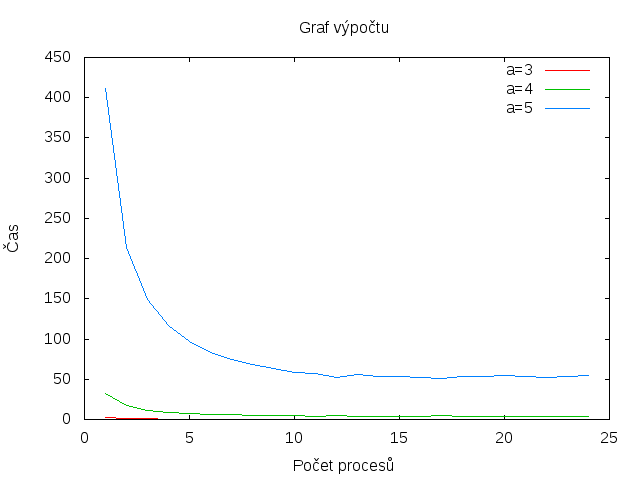
\includegraphics[width=1\textwidth]{../data/star_logs/graf_all.png}
  \caption{Graf všech výpočtů}
  \label{fig:con}
\end{figure}

Rozdíl mezi měřeními je dostatečný. Problém nastává pro malé časy výpočtu, které mají větší režijní čas než čas výpočtu. Pro porovnání je v následujících grafech vyneseno lineární zrychlení, kterému se zvolení řešení blíží.

\begin{figure}[H]
  \centering
    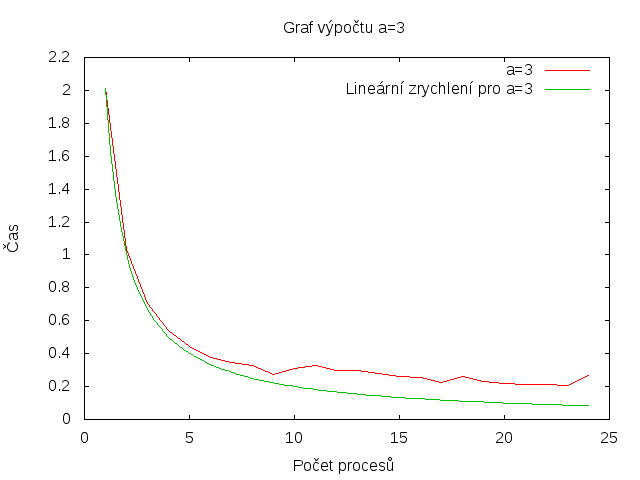
\includegraphics[width=1\textwidth]{../data/star_logs/graf3.png}
  \caption{Graf výpočtu pro $a=3$}
  \label{fig:tre}
\end{figure}

\begin{figure}[H]
  \centering
    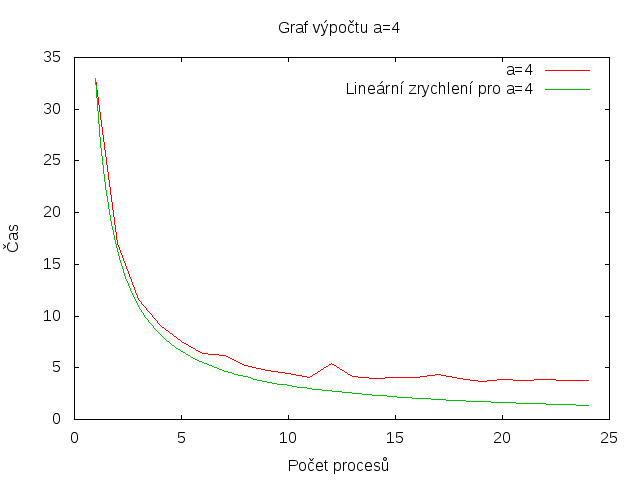
\includegraphics[width=1\textwidth]{../data/star_logs/graf4.png}
  \caption{Graf výpočtu pro $a=4$}
  \label{fig:fou}
\end{figure}

\begin{figure}[H]
  \centering
    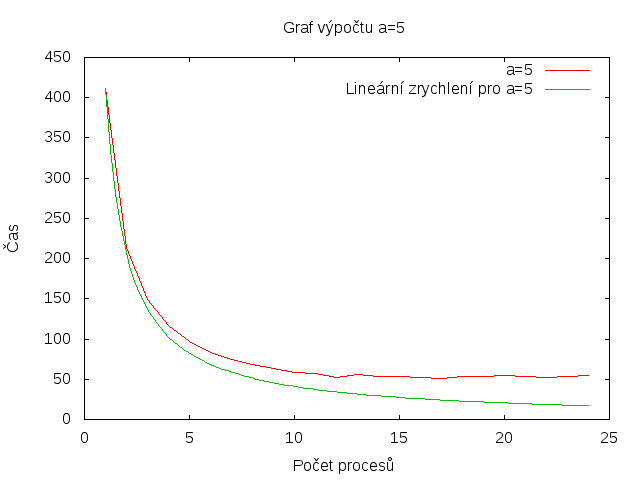
\includegraphics[width=1\textwidth]{../data/star_logs/graf5.png}
  \caption{Graf výpočtu pro $a=5$}
  \label{fig:fiv}
\end{figure}

Dle grafu je vidět, že se řešení blíží lineárnímu zrychlení. Je otázka, zdali doba výpočtu neklesá kvůli zatížení sítě či nějakému jinému technickému řešení.

\section{Závěr}

Je nutné zmínit, že jsme pro výpočet museli použít jen Ethernet. Maximální počet procesorů byl 24. Je otázka, zdali bychom při vypočtu narazili na maximum procesorů, které je možné použít. Teoreticky řešení může mít maximálně ${n \choose a}$ procesorů. Lepší detail by nám teoreticky prozradili izometrické funkce. Nicméně už s počtem procesorů 24 (pro námi zvolenou velikost problému) narážíme na praktické omezení.

\end{document}
